\section{\textbf{RELATED WORK}}\label{sec:RELATED WORK}

A predecessor of MPAT, named HAT (developed in the FICONTENT
2 project) has already been used to provide a childfriendly
sub-site for a German public broadcaster. The HbbTV
Application Toolkit (HAT) is an easy and cost-efficient way
for content creators to produce HbbTV applications. It is based
on the WordPress concept of providing tested templates and
components so content creators have an easy migration path.
For producing TV content, HAT only requires the same skill
set as for web page creation. Due to the separation of layout
templates and content, content creators can focus on their
content on screen without worrying about styles or maintaining
the required corporate design. These are already optimized for
TV use and ensure that an application created with HAT will
follow established rules for TV application development and
usage [3].
















 Figure \ref{fig:Use-case-Diagram}.

\begin{figure}[!ht]
	\centering
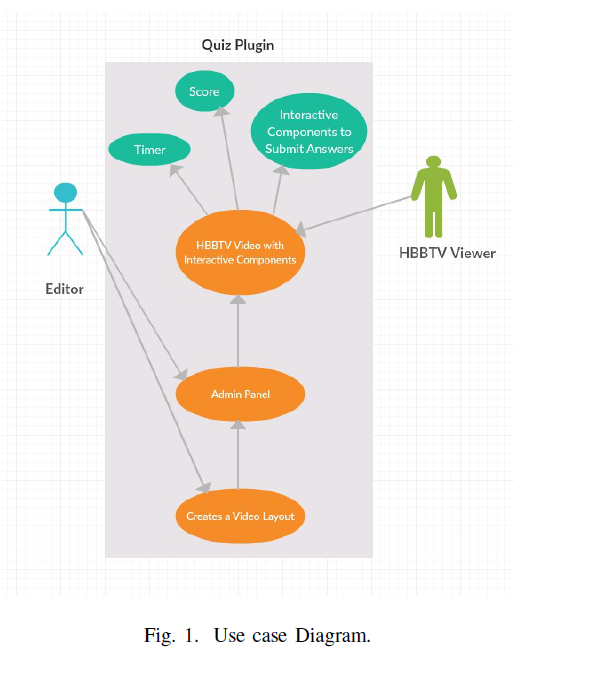
\includegraphics[scale=0.6]{figures/Use-case-Diagram.png}\\
	\caption{Use case Diagram }
	\label{fig:Use-case-Diagram}
\end{figure}
 

 
    